\chapter{Dise\~no}

\section{Diseño de la WSN}

\subsection{Conexión Física de la WSN}
La interconexión de los componentes clave en cada nodo sensor de la red inalámbrica de sensores (WSN) se llevará a cabo de manera precisa y adecuada para garantizar la operación coherente del sistema, como se muestra a continuación:
\begin{itemize}
\item \textbf{Microprocesador Arduino Pro Micro:}
\\El microprocesador Arduino Pro Micro, actuando como el cerebro de cada nodo sensor, establecerá conexiones directas a través de sus pines GPIO con cada uno de los sensores y módulos para la recopilación y procesamiento de datos. Además, se interconectará con el módulo LoRa UART para la transmisión inalámbrica de información.
\item \textbf{Sensores Específicos:}
\\El termistor LM35, destinado a medir la temperatura, será conectado a los pines analógicos del Arduino Pro Micro, garantizando una lectura precisa y oportuna de las condiciones ambientales. 
\\El módulo GPS Neo-6M, crucial para la geolocalización, se integrará a través de conexiones seriales, permitiendo al Arduino interpretar y registrar las coordenadas geográficas. 
\item \textbf{Comunicación Inalámbrica:}
\\El módulo LoRa UART 868/915 MHz establecerá una conexión serial con el Arduino Pro Micro, permitiendo la comunicación bidireccional entre los nodos sensores y la estación base. Esto facilitará la transmisión de datos y comandos, asegurando una coordinación efectiva dentro de la red.
\\La antena WiFi estará conectada directamente a la cámara trampa PR-700. Esta conexión permitirá que la cámara trampa se una a la red local a través de WiFi para la transmisión eficiente de imágenes y videos. La cámara trampa estará equipada con la capacidad de conectarse a una red WiFi, y la antena facilitará esta conexión para garantizar una transferencia de datos rápida y confiable.
\item \textbf{Almacenamiento:}
\\La memoria MicroSD a través del módulo MicroSD Card Adapter (modelo MLMSD), implementada como soluciones de almacenamiento local, se conectará al Arduino Pro Micro a través de interfaces SPI (Serial Peripheral Interface). Esto posibilitará un acceso rápido y eficiente para escribir y leer datos, garantizando la efectividad en la gestión de la información recopilada por los sensores distribuidos.
\item \textbf{Fuente de Energía:}
\\Las baterías recargables, conectadas a través de sistemas de gestión de energía, suministrarán la potencia necesaria al Arduino Pro Micro y sus componentes asociados. La eficiencia energética será clave para mantener la autonomía de los nodos sensores durante operaciones prolongadas.
\\También se incorporarán baterías a la cámara trampa PR-700 para garantizar su operación autónoma. Estas baterías proporcionarán la energía necesaria para el funcionamiento continuo de la cámara, asegurando la captura de imágenes y videos en diversas condiciones y entornos.
\end{itemize}
Esta configuración física(\hyperref[diseñowsn]{Figura \ref{diseñowsn}}) garantizará una interconexión robusta y eficiente, permitiendo que cada nodo sensor desempeñe sus funciones específicas de manera coordinada y efectiva dentro de la WSN.
\begin{figure}[H]
    \centering
    \includegraphics[width=1\linewidth,height=0.55\textheight]{imagenes/DiseñoWSN.jpg}
    \caption{Diseño de la WSN.}
    \label{diseñowsn}
\end{figure}
\subsection{Lenguaje de Programación de la WSN}
El lenguaje de programación seleccionado para el desarrollo de la WSN será Arduino IDE, dada su accesibilidad y versatilidad en la programación de microcontroladores. Esta elección facilita la implementación de algoritmos y la gestión de la comunicación entre los nodos de la red. A continuación, se detallan las principales librerías que se utilizarán en el desarrollo:
\begin{itemize}
\item \textbf{SoftwareSerial:} Será utilizada para establecer comunicación serial con componentes que requieran un puerto de comunicación adicional. Facilitará la conexión con módulos y dispositivos que no estén directamente conectados a los pines de hardware de comunicación serial \cite{sslibrary}.
\item \textbf{LoRa by Sandeep Mistry:} Se empleará para la implementación de la comunicación inalámbrica mediante la tecnología LoRa. Permitirá la transmisión de datos de manera eficiente y de largo alcance entre los nodos de la WSN, contribuyendo a la formación de un enjambre coordinado \cite{loralibrary}.
\item \textbf{TinyGPS:} Se aplicará para la interfaz con los módulos GPS. Facilitará la decodificación de datos de ubicación y simplificará el proceso de geolocalización en los nodos de la red \cite{tinygpslibrary}.
\item \textbf{SD:} La librería SD se utilizará para la gestión de la tarjeta MicroSD en los nodos que integran almacenamiento. Facilitará la lectura y escritura de datos en las tarjetas, permitiendo el almacenamiento local de información recolectada por los sensores \cite{sdlibrary}.
\end{itemize}

\newpage
\section{Diseño de los Drones }
El diseño de los drones desempeña un papel fundamental en el éxito de este proyecto. Cada elemento, desde el chasis hasta los componentes de propulsión y la fuente de energía, se utilizarán para garantizar un rendimiento óptimo y una adaptabilidad a las condiciones específicas del entorno de monitoreo.
\subsection{Estructura Física}
La estructura física de los drones se basará en un cuadricóptero, caracterizado por su configuración de cuatro rotores en disposición diagonal. Se ha seleccionado el chasis del kit S500 de la marca Readytosky, conocido como \textquotedbl{}engranaje\textquotedbl{}. Este chasis, fabricado en fibra de carbono, ofrece una combinación ideal de resistencia y ligereza para optimizar el rendimiento del dron en operaciones de vuelo.\\
Con dimensiones de 11.42 pulgadas de longitud, 7.09 pulgadas de ancho y 2.36 pulgadas de altura, el chasis proporciona un equilibrio adecuado entre tamaño compacto y capacidad para albergar los componentes esenciales. La distancia entre ejes de 19.685 pulgadas contribuye a la estabilidad del dron.\\
La configuración sugerida del kit S500 incluye un peso total con tren de aterrizaje de 15.87 oz. Para la propulsión, se recomiendan motores sin escobillas en el rango de tamaños 2212-2216, junto con hélices de 10\textquotedbl{}-12\textquotedbl{}. La batería sugerida abarca desde 3S a 4S con capacidades de 2200mAh a 5200mAh, y se sugiere un controlador de velocidad (ESC) en el rango de 20A-40A.
Estas especificaciones brindan flexibilidad para adaptar el dron a los requisitos específicos del proyecto. Además, que este fabricado en fibra de carbono garantiza durabilidad y resistencia estructural, elementos esenciales para operaciones en entornos desafiantes.
\subsection{Fuente de Energía}
La energía necesaria para alimentar el dron se suministrará a través de una batería de polímero de litio (LiPo) 3S con una capacidad de 5000mAh y una clasificación de voltaje de 11.1V. Este tipo de batería proporciona una combinación óptima de potencia y peso para garantizar un rendimiento eficiente durante las operaciones de monitoreo.\\
La capacidad de 5000mAh ofrece una duración de vuelo considerable, lo que es esencial para misiones de monitoreo prolongadas. El voltaje de 11.1V se adapta a la configuración del sistema, brindando la potencia necesaria para los motores y otros componentes electrónicos del dron.\\
El conector XT-60 asegura una conexión segura y confiable entre la batería y el sistema eléctrico del dron. Este conector es conocido por su eficiencia en la transmisión de corriente, minimizando pérdidas y garantizando un suministro estable de energía durante la operación.\\
La elección de esta batería LiPo específica se basa en su equilibrio entre capacidad, voltaje y compatibilidad con el sistema eléctrico del dron. Esto contribuye a la eficiencia general del dron, asegurando una fuente de energía confiable para las diversas funciones del sistema durante las misiones de vuelo.
\subsection{Componentes para Volar el Dron}
El sistema de propulsión del dron estará compuesto por componentes de alta calidad que garantizan un rendimiento confiable y eficiente durante las operaciones de vuelo. A continuación se detallan los elementos clave de este sistema:
\begin{itemize}
\item \textbf{Par de Hélices 1045 de Carbono y Nylon para F450/F550:} Cada ala del dron estará equipada con un par de hélices 1045 fabricadas con una combinación de carbono y nylon. Estas hélices proporcionan un equilibrio óptimo entre resistencia y ligereza, contribuyendo a la eficiencia del vuelo y asegurando una generación de empuje adecuada.
\item \textbf{Motor sin Escobillas 2212 920KV (actualización CCW):} El sistema de propulsión contará con motores sin escobillas de alta calidad, específicamente el modelo 2212 con una clasificación de 920KV y configuración de rotación antihoraria (CCW). Estos motores ofrecen un rendimiento potente y eficiente, adecuado para las demandas de misiones de monitoreo y vuelo estable.
\item \textbf{Pixhawk 2.4.8 Autopiloto Controlador PM PPM PX4 Ardupilot:} El corazón del sistema de vuelo será el controlador Pixhawk 2.4.8, que opera bajo los sistemas PX4 y Ardupilot. Este autopiloto proporciona funciones avanzadas de control de vuelo, navegación y estabilización. Su capacidad para integrarse con sistemas de posicionamiento, como el GPS Here+, garantiza una precisión y confiabilidad superiores durante las misiones de monitoreo.
\end{itemize}
La combinación de estas propelas, motores y el sistema de control autopiloto como se puede ver en la \hyperref[diseñodron]{Figura \ref{diseñodron}} proporciona una configuración integral que respalda un vuelo controlado y preciso del dron durante las misiones de vuelo.
\begin{figure}[H]
\centering
\includegraphics[width=1\textwidth]{imagenes/DiseñoDron.jpg}
\caption{Diseño del dron.}
\label{diseñodron}
\end{figure}

\newpage
\section{Diseño del Enjambre de Drones}
El diseño del enjambre de drones para el monitoreo de especies en peligro de extinción representa la culminación de un análisis exhaustivo y una planificación meticulosa. Este concepto innovador fusiona la eficiencia individual de los drones con una coordinación inteligente y descentralizada para abordar los desafíos críticos de la conservación biológica. En este diseño, cada dron individual se convierte en un nodo esencial en una red autónoma y colaborativa. La integración de microordenadores y transceptores de comunicación, potenciará la capacidad de procesamiento y la conexión inalámbrica entre los drones, respectivamente. Este enfoque permitirá una ejecución de algoritmos avanzados y una coordinación en tiempo real entre los miembros del enjambre.
\subsection{Arquitectura Física}
La arquitectura física del enjambre de drones aprovechará la sólida configuración de cuadricópteros, heredada del diseño individual de drones descrito previamente. Que se conforma por el chasis del kit S500 de fibra de carbono, baterías LiPo 3S, etc.\\
La evolución hacia un enjambre inteligente implica la incorporación estratégica de componentes clave. A la estructura existente se le añadirán un microordenador Raspberry Pi 4 y un transceptor LoRa UART 868MHz/915MHz. Estos elementos, cuidadosamente seleccionados durante el análisis, elevan la funcionalidad de cada dron a una capacidad de procesamiento superior y a una comunicación eficiente entre ellos.\\
En el contexto del diseño del enjambre de drones, la integración del microordenador Raspberry Pi 4 representa un avance significativo en la capacidad de procesamiento del sistema. Este componente actúa como el cerebro central de cada dron, brindando la potencia computacional necesaria para ejecutar algoritmos avanzados. La inclusión de Raspberry Pi 4 no solo permite un procesamiento más eficiente de los datos recopilados por los sensores del dron, sino que también habilita la implementación de algoritmos complejos para tareas como la navegación autónoma y la toma de decisiones en tiempo real. Además, la introducción del transceptor LoRa UART 868MHz/915MHz mejora significativamente la capacidad de comunicación entre los drones del enjambre. La frecuencia LoRa seleccionada (868MHz/915MHz) garantiza una cobertura adecuada y una transmisión confiable de datos, elementos cruciales para el éxito de las misiones de monitoreo en entornos diversos y desafiantes. \\
En conjunto, la combinación de Raspberry Pi 4 y el transceptor LoRa fortalece la inteligencia colectiva del enjambre, mejorando su capacidad para ejecutar misiones de manera colectiva. Así, la estructura física del enjambre fusiona la confiabilidad estructural del diseño individual del dron con la potencia adicional de estos nuevos componentes, creando una plataforma integral que maximiza la inteligencia colectiva del enjambre para afrontar con eficacia las misiones de este proyecto.

\subsection{Algoritmos de Comunicación}
En el diseño del sistema de comunicación para el enjambre de drones, se implementarán algoritmos que permitan una transmisión eficiente de instrucciones desde la estación base hasta los drones individuales. Este enfoque optimiza el proceso al evitar la necesidad de enviar instrucciones directamente a cada dron, delegando esta tarea al dron líder. A continuación, se describen los algoritmos clave para facilitar esta comunicación jerárquica:
\begin{enumerate}
\item \textbf{Instrucciones de la estación base al dron líder:} La estación base enviará instrucciones y comandos generales al dron líder a través de la red de comunicación establecida.
Estas instrucciones pueden incluir cambios en la ruta de vuelo, ajustes en la altitud, solicitudes de recopilación de datos específicos, entre otros.
\item \textbf{Transmisión de instrucciones del dron líder a los drones subordinados:} El dron líder, al recibir las instrucciones de la estación base, actúa como el punto central de coordinación dentro del enjambre.
Utilizando el transceptor LoRa, el dron líder transmite las instrucciones a los demás drones de manera eficiente, asegurando una comunicación rápida y confiable.
Este proceso se realiza de manera iterativa y continua, permitiendo una actualización constante de las instrucciones a medida que la misión avanza.
\item \textbf{Confirmación de recepción y ejecución:} Cada dron, al recibir las instrucciones, envía una confirmación al dron líder para indicar la recepción exitosa.
Una vez que el dron líder recibe confirmaciones de todos los drones subordinados, puede informar a la estación base sobre el estado de la transmisión y la ejecución de las instrucciones.
\item \textbf{Gestión de conflictos y replanificación:}
En caso de que un dron subordinado encuentre un conflicto o imprevisto durante la ejecución de las instrucciones, informará al dron líder.
El dron líder puede, entonces, replanificar la misión, ajustando las instrucciones y transmitiendo las actualizaciones correspondientes al enjambre.
\end{enumerate}
Este enfoque jerárquico en la comunicación permite una mayor eficiencia operativa, ya que centraliza la gestión de instrucciones en el dron líder, reduciendo la carga de comunicación desde la estación base y mejorando la sincronización del enjambre durante las misiones de monitoreo. Además, la implementación de confirmaciones y mecanismos de gestión de conflictos contribuye a la robustez y adaptabilidad del sistema en entornos dinámicos.

\subsection{Programación de Rutas}
La programación de rutas es un componente crítico en el despliegue eficiente del enjambre de drones para el monitoreo de especies en peligro de extinción. Para esta tarea, se empleará Mission Planner 1.3.81, una plataforma de planificación de vuelo robusta y versátil. A continuación, se detallan los pasos clave y consideraciones para la programación de rutas utilizando esta herramienta:
\begin{enumerate}
\item \textbf{Configuración inicial:} Antes de iniciar la programación de rutas, se realizará una configuración inicial en Mission Planner. Esto incluirá la conexión de la estación base con el dron líder a través de la interfaz de comunicación establecida.
\item \textbf{Definición de puntos de interés:} Se identificarán y marcarán los puntos de interés críticos en el área de monitoreo, como hábitats de especies en peligro o zonas específicas que requieran mayor atención.
Estos puntos servirán como referencias para la planificación de rutas y la asignación de tareas específicas a los drones.
\item \textbf{Creación de rutas autónomas:} Utilizando Mission Planner, se diseñarán rutas autónomas para cada dron en el enjambre. Estas rutas se basarán en la ubicación de los puntos de interés y se optimizarán para cubrir eficientemente el área de monitoreo.
Se programarán altitudes específicas, velocidades de vuelo y patrones de mapeo para garantizar una cobertura completa y detallada del terreno.
\item \textbf{Implementación de puntos de control:} Se establecerán puntos de control a lo largo de las rutas para garantizar la precisión y estabilidad del vuelo. Estos puntos permitirán ajustes en tiempo real durante la misión.
Los puntos de control también facilitarán la coordinación entre los drones, asegurando una distribución equitativa de las tareas y evitando superposiciones no deseadas.
\item \textbf{Verificación y simulación:} Antes de la ejecución en campo, se verificarán las rutas programadas y se realizarán simulaciones en Mission Planner. Esto permite identificar posibles problemas y optimizar la eficiencia de las rutas antes del despliegue real.
\item \textbf{Carga de misiones a los drones:} Una vez finalizada la programación y verificación, las misiones planificadas se cargarán en cada dron del enjambre. Esto se realizará de manera centralizada desde la estación base, asegurando consistencia en las instrucciones.
\item \textbf{Monitoreo en tiempo real:} Durante la ejecución de la misión, Mission Planner proporcionará herramientas para monitorear en tiempo real la posición de cada dron, la cobertura del área y cualquier desviación con respecto a la ruta planificada.
\end{enumerate}
\begin{figure}[H]
    \centering
    
\includegraphics[width=0.5\linewidth]{imagenes/MissionPlanner.png}
    \caption{Logo de Mission Planner.}
\end{figure}
\newpage
\noindent La adición de estos componentes al diseño de un dron individual, como se puede ver en la \hyperref[diseñoenjambre]{Figura \ref{diseñoenjambre}}, les permitirá a los drones comportarse de una forma colectiva simulando el comportamiento de un enjambre.
\newline
\begin{figure}[H]
    \centering
    \includegraphics[width=1\linewidth,height=0.5\textheight]{imagenes/DiseñoEnjambre.jpg}
    \caption{Diseño del enjambre de drones.}
    \label{diseñoenjambre}
\end{figure}

\newpage
\section{Diseño del Dominio en la Nube}
Para el diseño en la nube, debemos de tener en cuenta varios servicios que nos interesan adquirir, serán una mezcla de varios servicios que pueden interactuar unos con otros para automatizar ciertos procesos como por ejemplo, el ordenamiento de los datos por fechas y que se clasifiquen dependiendo del tipo de archivo que sea, como puede ser audio, vídeo, imágenes o simplemente datos; también podremos programar ciertas visualizaciones de los datos obtenidos y procesarlos de manera que tengamos datos limpios (nos referimos a datos limpios como los datos que nos son útiles para procesar en visualizaciones, análisis o similar, sin presentar inconsistencias, valores repetidos o datos incorrectos). 
Uno de los servicios que nos ofrece AWS es Cognito, que lo usaremos para autenticación de los usuarios que tendrán acceso a la base de datos, por lo que vamos a explicarlo a continuación.
\subsection{Amazon Cognito}
Amazon Cognito es una plataforma de identidad para aplicaciones web y móviles. Es un directorio de usuarios, un servidor de autenticación y un servicio de autorización para los tokens y credenciales de AWS de acceso de OAuth 2.0. Con Amazon Cognito, puede autenticar y autorizar a los usuarios desde el directorio de usuarios integrado, desde el directorio empresarial y desde proveedores de identidad de consumidores como Google y Facebook.
OAuth 2.0 es un protocolo de autorización y NO un protocolo de autenticación, utiliza tokens de acceso\cite{128}. \\
Los dos componentes siguientes componen Amazon Cognito. Funcionan de forma independiente o en conjunto, en función de las necesidades de acceso de los usuarios.

\subsubsection{Grupo de Usuarios}

\begin{figure}[hbtp]
\centering
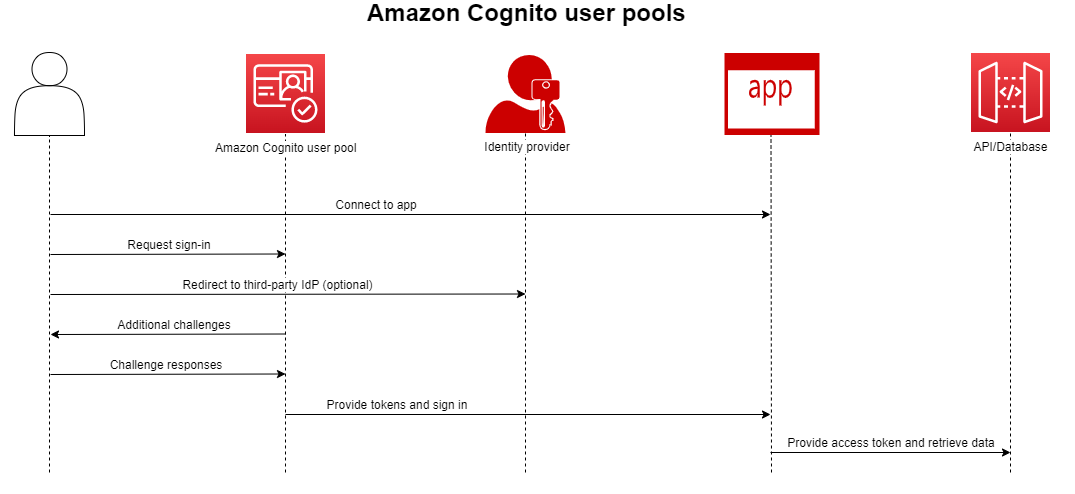
\includegraphics[width=.75\textwidth]{imagenes/ac_user_pool.png}
\caption{Grupo de Usuarios de Amazon Cognito diagrama de funcionamiento}
\end{figure}

\noindent Sirve para crear un grupo de usuarios cuando quiera autenticar y autorizar a los usuarios a la aplicación o la API. Los grupos de usuarios son un directorio de usuarios con funciones de creación, administración y autenticación de usuarios automáticas e impulsadas por el administrador. 
Los grupos de usuarios no requieren la integración con un grupo de identidades. Desde un grupo de usuarios, puede emitir JSON Web Token (JWT) autenticados directamente a una aplicación, un servidor web o una API.


\noindent Un grupo de usuarios de Amazon Cognito es un directorio de usuarios. Con un grupo de usuarios, los usuarios pueden iniciar sesión en su aplicación web o móvil por medio de Amazon Cognito o federarse mediante un IdP de terceros. Los usuarios federados y locales tienen un perfil de usuario en el grupo de usuarios.
Los grupos de usuarios de Amazon Cognito aceptan tokens y afirmaciones de IdP de terceros y recopilan los atributos de los usuarios en un JWT(JSON Web Token) que emite a la aplicación. Puede estandarizar la aplicación en un conjunto de JWT mientras Amazon Cognito gestiona las interacciones con los IdP y asigna las reclamaciones a un formato de token central. 

\subsubsection{Grupos de Identidades}

\begin{figure}[h]
\centering
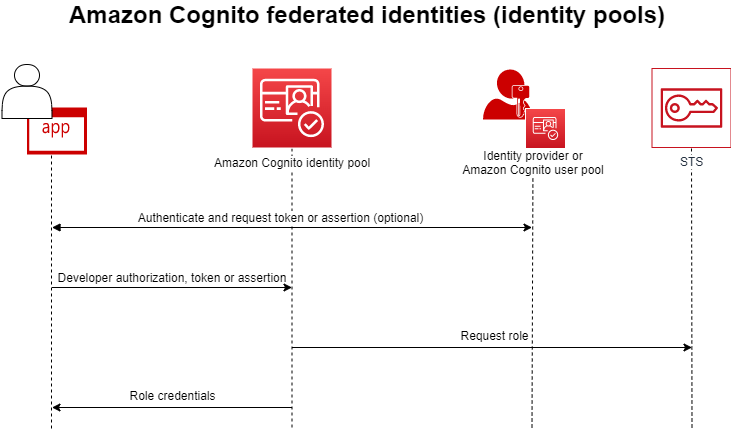
\includegraphics[width=.75\textwidth]{imagenes/ac_fed_pool.png}
\caption{Grupo de Usuarios de Amazon Cognito diagrama de funcionamiento}
\end{figure}

Configurar un grupo de identidades de Amazon Cognito cuando desee autorizar a los usuarios autenticados o anónimos a acceder a los recursos de AWS. Un grupo de identidades emite credenciales de AWS para que la aplicación proporcione recursos a los usuarios. Puede autenticar a los usuarios con un proveedor de identidades de confianza, como un grupo de usuarios. También puede emitir, opcionalmente, credenciales para los usuarios invitados. Los grupos de identidades utilizan un control de acceso basado en roles y atributos para administrar la autorización de los usuarios para acceder a los recursos de AWS.

Se utiliza Amazon Cognito para autenticar al usuario y, a continuación, concederle acceso a un Servicio de AWS.
\begin{enumerate}
\item El usuario de la aplicación inicia sesión a través de un grupo de usuarios y recibe los tokens de OAuth 2.0.
\item La aplicación intercambia un token de grupo de usuarios por un grupo de identidades para obtener credenciales de AWS temporales que puede usar con las API de AWS y la AWS Command Line Interface (AWS CLI).
\item La aplicación asigna la sesión de credenciales al usuario y proporciona acceso autorizado a Servicios de AWS como Amazon S3 y Amazon DynamoDB.
\end{enumerate}

En Amazon Cognito, la obligación de seguridad de la nube del modelo de responsabilidad compartida cumple con SOC 1-3, PCI DSS, ISO 27001 e HIPAA-BAA. Puede diseñar la seguridad en la nube en Amazon Cognito para que cumpla con SOC1-3, ISO 27001 e HIPAA-BAA, pero no con DSS de PCI. 


\noindent Un grupo de identidades es un conjunto de identificadores o identidades únicas que se asignan a los usuarios o invitados y se autoriza a recibir credenciales temporales de AWS. Al presentar una prueba de autenticación en un grupo de identidades en forma de afirmaciones fiables de un proveedor de identidades sociales (IdP) de SAML 2.0, OpenID Connect (OIDC) u OAuth 2.0, se asocia al usuario con una identidad del grupo de identidades. El token que el grupo de identidades crea para la identidad puede recuperar las credenciales de sesión temporales de AWS Security Token Service (AWS STS).

Para complementar las identidades autenticadas, también se puede configurar un grupo de identidades para autorizar el acceso de AWS sin autenticación de IdP. Puede ofrecer su propia prueba de autenticación personalizada o no tener autenticación. Puede conceder credenciales de AWS temporales a cualquier usuario de la aplicación que las solicite, con identidades no autenticadas.

\subsubsection{Control de Acceso con Base en Roles}
Cuando el usuario pasa las reclamaciones al grupo de identidades, Amazon Cognito elige el rol de IAM que solicita. Para personalizar los permisos del rol según las necesidades, se aplican las políticas de IAM a cada rol. Amazon Cognito puede solicitar un rol predeterminado, un rol basado en reglas que consultan las reclamaciones del usuario o un rol basado en la suscripción al grupo del usuario en un grupo de usuarios. También puede configurar la política de confianza de roles para que IAM confíe solo en el grupo de identidades para generar sesiones temporales\cite{129}.


\subsection{AWS Identity and Access Management}

AWS Identity and Access Management (IAM) es un servicio web que ayuda a controlar de forma segura el acceso a los recursos de AWS. Con IAM, se puede administrar de forma centralizada los permisos que controlan a qué recursos de AWS pueden acceder los usuarios. Se utiliza IAM; para controlar quién está autenticado (ha iniciado sesión) y autorizado (tiene permisos) para utilizar recursos.

Cuando se crea una Cuenta de AWS, se comienza con una identidad de inicio de sesión que tiene acceso completo a todos los recursos y Servicios de AWS de la cuenta. Esta identidad recibe el nombre de usuario raíz de la Cuenta de AWS y se accede a ella iniciando sesión con el email y la contraseña que utilizó para crear la cuenta. Se recomienda no utilizar la cuenta raíz para hacer actividades cotidianas\cite{130}.

Los 2 servicios anteriores únicamente son para autenticación lo cual es una herramienta muy importante ya que los datos que vamos a almacenar, aunque no sean confidenciales, sí son muy importantes y servirán para los análisis profesionales de los biólogos; y es destacable la forma de autenticación y verificación de las personas que se van a encargar del almacenamiento de los datos (nosotros mismos contaremos con los roles de administradores), ya que nosotros mismos nos encargaremos de darle seguridad e integridad a los datos para que no tengan vulnerabilidades los accesos y no entren intrusos a la información.

\subsection{Amazon Lambda}

AWS Lambda es un servicio informático que permite ejecutar código sin aprovisionar ni administrar servidores. Con Lambda, lo único que tiene que hacer es suministrar el código en uno de los tiempos de ejecución de lenguaje compatibles con Lambda \cite{131}.

Con el servicio de lambda podemos automatizar el proceso de limpieza de datos y el propio almacenamiento en la base de datos que vamos a utilizar, y podemos utilizar diferentes lenguajes de programación como Java o Python para procesar los datos.

\subsection{Amazon Simple Storage Service (Amazon S3)}

Amazon Simple Storage Service (Amazon S3) es un servicio de almacenamiento de objetos que ofrece escalabilidad, disponibilidad de datos, seguridad y rendimiento, se utiliza Amazon S3 para almacenar y proteger cualquier cantidad de datos para diversos casos de uso, tales como lagos de datos, sitios web, aplicaciones móviles, copia de seguridad y restauración, archivado, aplicaciones empresariales, dispositivos IoT y análisis de big data.

Amazon S3 proporciona funciones de gestión para que pueda optimizar, organizar y configurar el acceso a los datos almacenados.



\begin{figure}[hbtp]
\centering
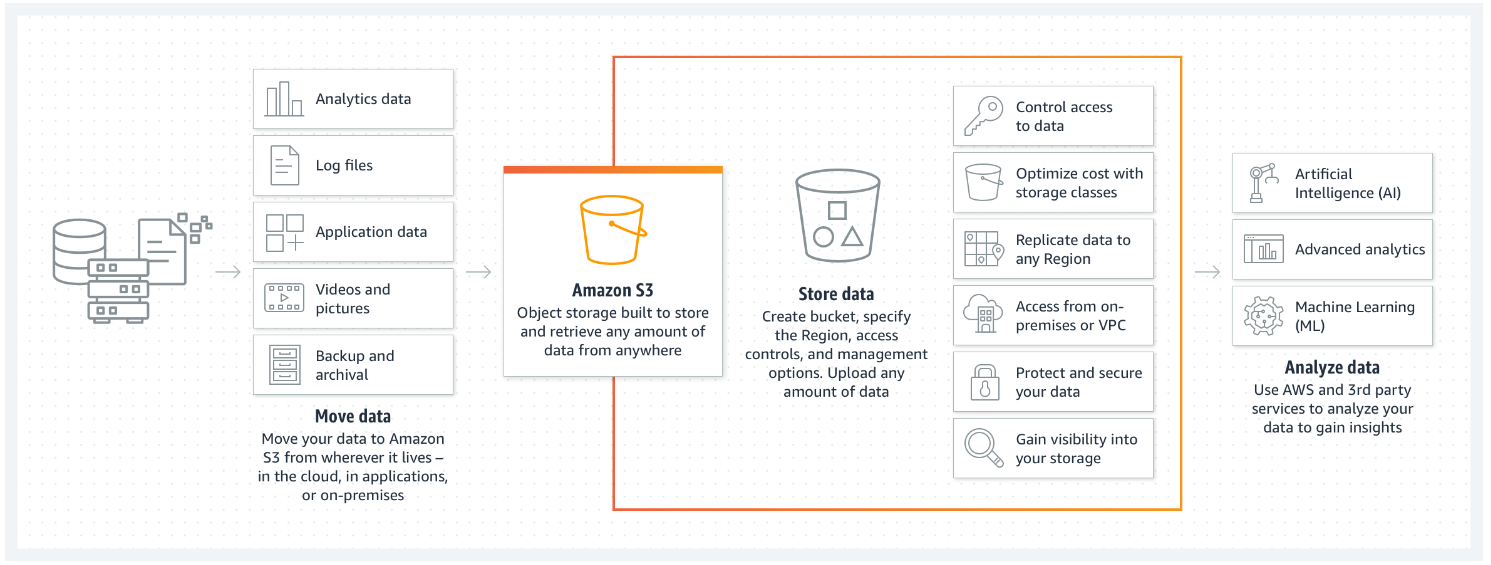
\includegraphics[width=\textwidth]{imagenes/s3.png}
\caption{Traslado de los datos a Amazon S3, administración de los datos almacenados en Amazon S3 y análisis de los datos con otros servicios de AWS. }
\end{figure}

El diagrama muestra cómo trasladar los datos a Amazon S3, administrar los datos almacenados en Amazon S3 y analizar los datos con otros servicios. Se muestran tres secciones de izquierda a derecha \cite{132}.

Amazon S3 ofrece varios tipos de almacenamiento diseñados para distintos casos de uso. Por ejemplo, puede almacenar datos de producción críticos en S3 Standard para obtener acceso frecuente, ahorrar costos al almacenar datos a los que se accede con poca frecuencia en S3 Standard-IA o S3 One Zone-IA, y archivar datos con los costos más bajos en S3 Glacier Instant Retrieval, S3 Glacier Flexible Retrieval y S3 Glacier Deep Archive.

También, se pueden instanciar páginas web en el servicio de de S3, por lo que nos será útil para cuando diseñemos la página web para visualización y acceso a los datos de usuarios que tengan permiso y acceso a ellos.

\subsection{Amazon DynamoDB}
Amazon DynamoDB es un servicio de base de datos NoSQL totalmente administrado que ofrece un rendimiento rápido y predecible, así como una perfecta escalabilidad. Permite delegar las cargas administrativas que supone tener que utilizar y escalar bases de datos distribuidas, para que no tengamos que preocuparnos del aprovisionamiento, la instalación ni la configuración del hardware, ni tampoco de las tareas de replicación, aplicación de parches de software o escalado de clústeres. DynamoDB también ofrece el cifrado en reposo, que elimina la carga y la complejidad operativa que conlleva la protección de información confidencial. 

Podemos crear tablas de base de datos capaces de almacenar y recuperar cualquier cantidad de datos, así como de atender cualquier nivel de tráfico de solicitudes. Se puede escalar la capacidad de rendimiento de las tablas para aumentarla o reducirla sin tiempos de inactividad ni reducción del desempeño.

\begin{figure}[hbtp]
\centering
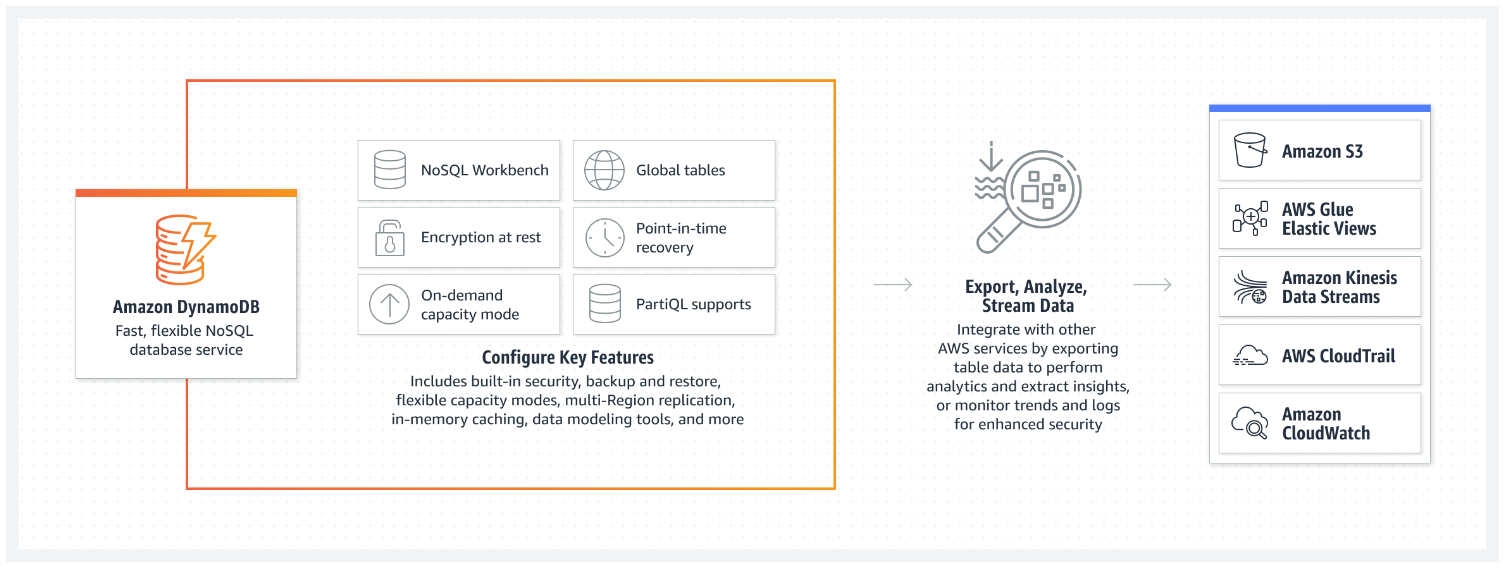
\includegraphics[width=\textwidth]{imagenes/dynamodb.png}
\caption{Características principales de Amazon DynamoDB y las integraciones con otros servicios de AWS}
\end{figure}


En el diagrama se muestran las características principales de Amazon DynamoDB y las integraciones con otros servicios de AWS. Se muestran tres secciones de izquierda a derecha.

Las características de importación y exportación de DynamoDB ayudan a mover, transformar y copiar cuentas de tablas de DynamoDB, o AWS. Se puede importar desde sus orígenes de S3 y puede exportar los datos de sus tablas de DynamoDB a Amazon S3 y utilizar servicios de AWS como Athena, Amazon SageMaker y AWS Lake Formation que son servicios que se pueden considerar introducir en algún momento para analizar los datos y extraer información procesable. También se puede importar datos directamente a nuevas tablas de DynamoDB para crear nuevas aplicaciones con un rendimiento de un milisegundo a escala, facilitar el uso compartido de datos entre tablas y cuentas, y simplificar sus planes de recuperación de desastres y continuidad empresarial \cite{133}.

\subsection{Amazon QuickSight}
Amazon QuickSight es una herramienta que nos ayudará a crear presentaciones gráficas sobre los datos que obtengamos, podremos utilizar diversas gráficas que nos ayudarán a una mejor visualización de los datos, serán más entendibles que simple texto plano y serán más amigables de entregar en reportes de análisis de datos.

Lo que estaremos usando serán estos servicios de almacenamiento, gestión y seguridad de datos. Es muy importante la conexión e integración de estos servicios ya que cada uno realizará una tarea en específico para lograr los objetivos de análisis de la especie a analizar.

El siguiente esquema es una representación gráfica de lo que vamos a hacer en el proyecto.

\begin{figure}[h]
\centering
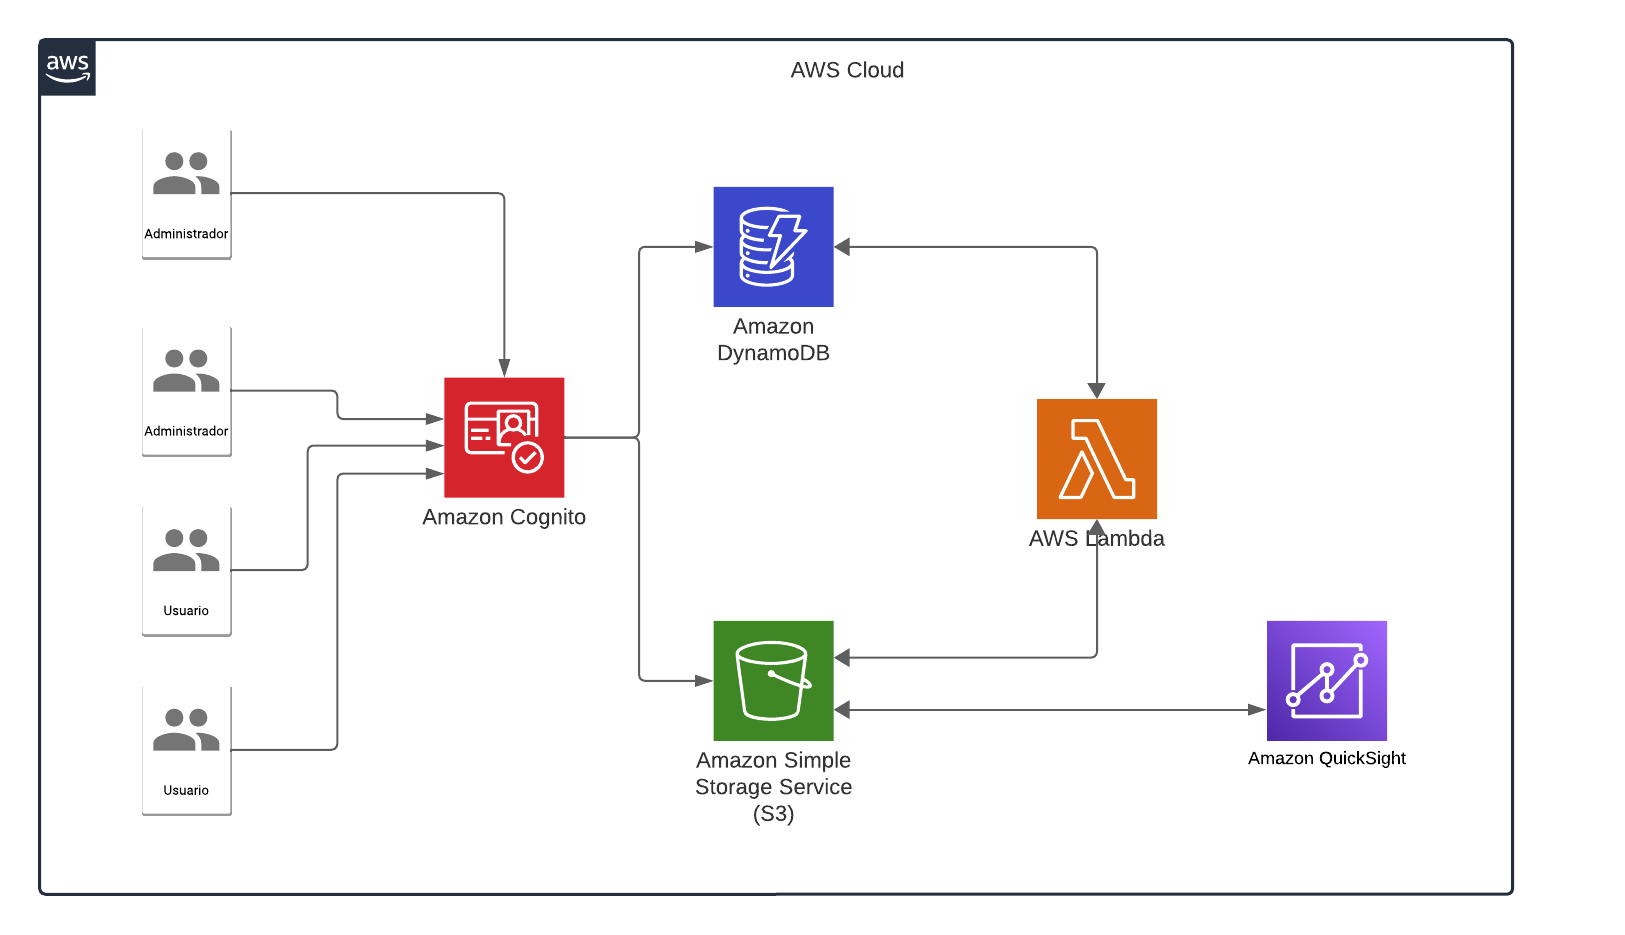
\includegraphics[width=\textwidth]{imagenes/diagrama.png}
\caption{Diagrama de bloques de los servicios que se consideran para el desarrollo del proyecto.}
\end{figure}

Habrán 2 administradores que serán los alumnos que desarrollarán el proyecto y tendrán todos los permisos, contaremos con 2 usuarios (depende como evolucione el proyecto se irán incluyendo más usuarios) los cuales no contarán con todos los permisos de escritura y únicamente contarán con los permisos de visualización de los datos, y estos 2 usuarios serán los asesores del proyecto. Usaremos el servicio de Amazon Cognito para la validación de identidades de los usuarios (se aplicará a los usuarios administradores y los usuarios normales), posteriormente usaremos 2 servicios de almacenamiento, el servicio de S3 lo usaremos como almacenamiento de todos los datos que involucran al proyecto, tales son archivos de video, imágen, audio, texto plano, gráficos, entre otros tipos de archivos, el servicio de DynamoDB será ocupado como la base de datos NoSQL en la cuál vamos a crear nuestras tablas NoSQL donde organizaremos nuestros archivos.

Es muy importante hacer la diferencia entre los servicios DynamoDB y S3, DynamoDB es una base de datos que se almacenan en caché y únicamente crearemos tablas NoSQL para identificación de archivos, por lo que para almacenar los datos necesitamos el servicio de S3 que será el lugar de almacenamiento de todos los archivos descritos anteriormente y también almacenaremos copias de seguridad y las propias tablas que generamos en DynamoDB.

Usaremos el servicio de Lambda que estará vinculado a los servicios de S3 y DynamoDB para procesar archivos. Con lo de procesar los datos nos referimos a la limpieza de los datos y almacenamiento automático de los datos. Ya que el servicio de Lambda nos ayuda a crear funciones que nos permitirán procesar los datos con diferentes lenguajes de programación, entre ellos podemos usar Java y Python.

El servicio de QuickSight únicamente lo tomamos para visualización de los datos, ya que es muy necesario interpretar de forma correcta los datos obtenidos por nosotros y crear gráficas o recursos visuales que nos ayuden a entender de forma más sencilla los datos limpios, aunque este servicio lo podemos reemplazar por el propio AWS Lambda o algún programa de manipulación de datos local como PowerBI u otros en línea como Tableau que se pueden colocar nuestros resultados en línea para consulta de terceros (esto es opcional y dependerá de los permisos de publicación de datos con las vinculaciones que tengamos con los biólogos).

\newpage
\section{Creación del Dominio en la Nube}
El dominio en la nube se elaboró con una cuenta de los alumnos que están desarrollando el proyecto y contiene la siguiente información.


\begin{figure}[h]
\centering
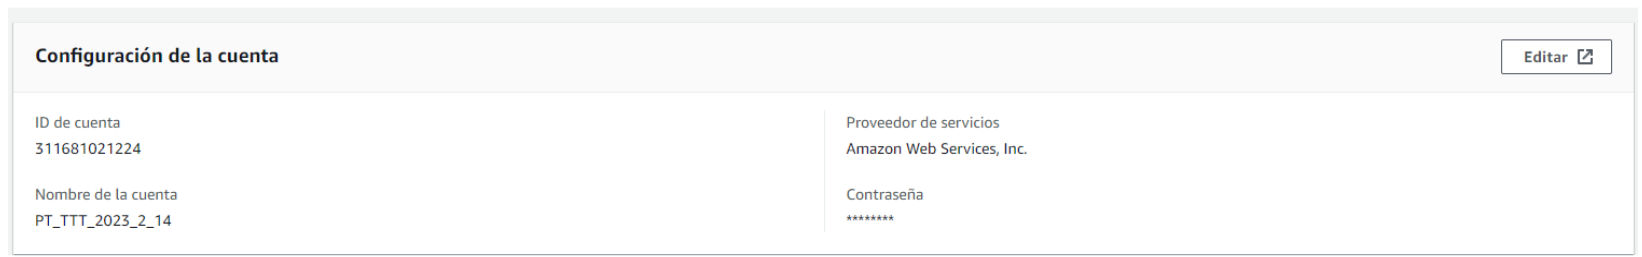
\includegraphics[width=\textwidth]{imagenes/cuenta.png}
\caption{Características del dominio en la nube.}
\end{figure}
\newpage

Ya creado el dominio, podemos observar la página de inicio y podemos empezar a usar los servicios; Es importante estar inspeccionando los precios de los servicios para estar informados sobre los movimientos que vamos haciendo y saber cuánto dinero es necesario pagar al final de la fecha de facturación.

\begin{figure}[h]
\centering
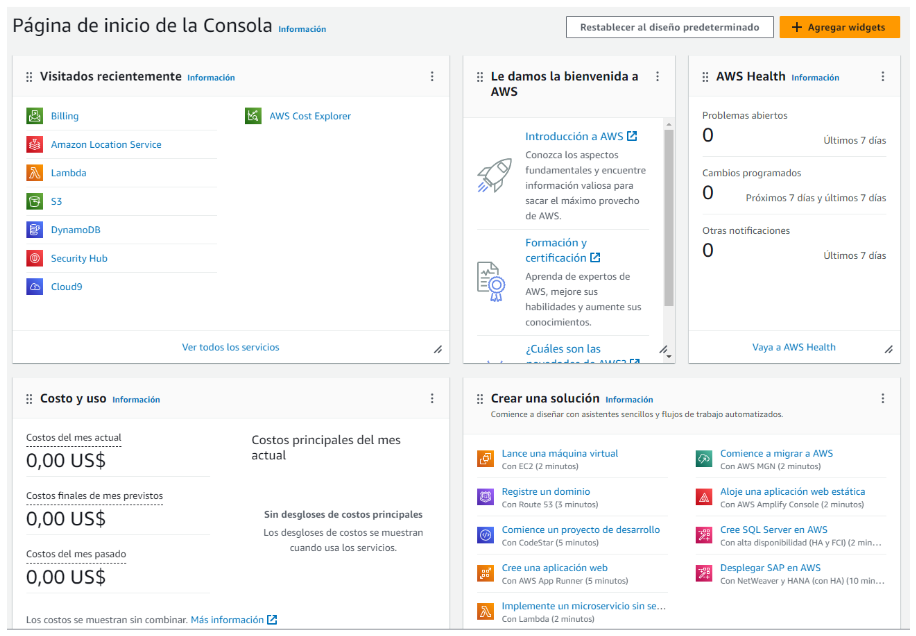
\includegraphics[width=0.8\textwidth]{imagenes/pag_principal.png}
\caption{Visualización de la página principal al iniciar sesión en AWS}
\end{figure}




